This chapter is divided in five sections. In section \ref{tresponto1} it is briefly discussed the proposed model for the temporal decorrelation. In section \ref{tresponto2} and \ref{tresponto3} it is presented the current chain of processing for the backscatter and coherence estimation using SENTINEL-1 multi-temporal series. In section \ref{tresponto4} it is discussed the input features that were chosen for the classification model based on the Random Forest algorithm and it's methods for accuracy validation. On the final section it is presented the Datasets that were used by \cite{Paolo} for the classification map generation.

\section{Temporal decorrelation model}
\label{tresponto1}
As mentioned in chapter 2, the temporal decorrelation model is given by:

\begin{equation}
    \rho(t) = (\rho_0 -\rho_{LT}) \exp{\left(-\left(t/{\tau}\right) ^2\right)} + \rho_{LT}
\end{equation}{}

Where $\rho_{LT}$ is the long term coherence and $\tau$ is the decorrelation decay factor. Both of these informations are useful for classification. It's worth mentioning that taking the limits to zero and infinity yields 1 and $\rho_{LT}$ respectively. 

Assuming that the acquisitions occur periodically, then the time is always a multiple of the period of acquisition, such that $t=nT$, where $T$ is the period of acquisition (6 days for the SENTINEL-1). 

Graphically different decorrelation decay factors can be seen in the figure \ref{fig:temporal decorrelation}. 

\begin{figure}[H]
    \centering
    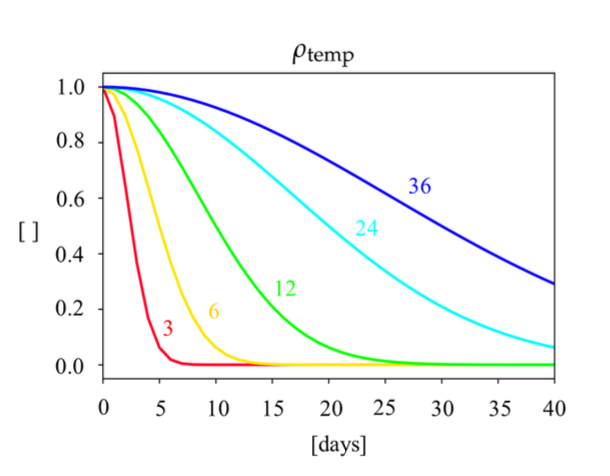
\includegraphics[width=0.7\linewidth]{Cap3/decay.png}
    \caption{Temporal Decorrelation for different decay factors \cite{Paolo} where each color indicates a different decay constant $\tau$ (show by the number above it).}
    \label{fig:temporal decorrelation}
\end{figure}

To extract these parameters, the data will be acquired and then this curve will be fitted for the different areas and these parameters will be extracted.

\section{Sentinel-1 processing chain}
\label{tresponto2}
After acquiring a series of $N$ wide-swaths the first step that must be done is the coregistration. The coregistration is a geometry transformation ( as shown in \cite{coregistration}) that takes the acquisitions and transform to what it would like if it would have been acquired in other position (this position is the SAR acquisition position that is closest to the average, this SAR acquisition is called the Master acquisition). The Figure \ref{fig:processing_chain} shows the processing chain for the SENTINEL-1 radar.

\begin{figure}[H]
    \centering
    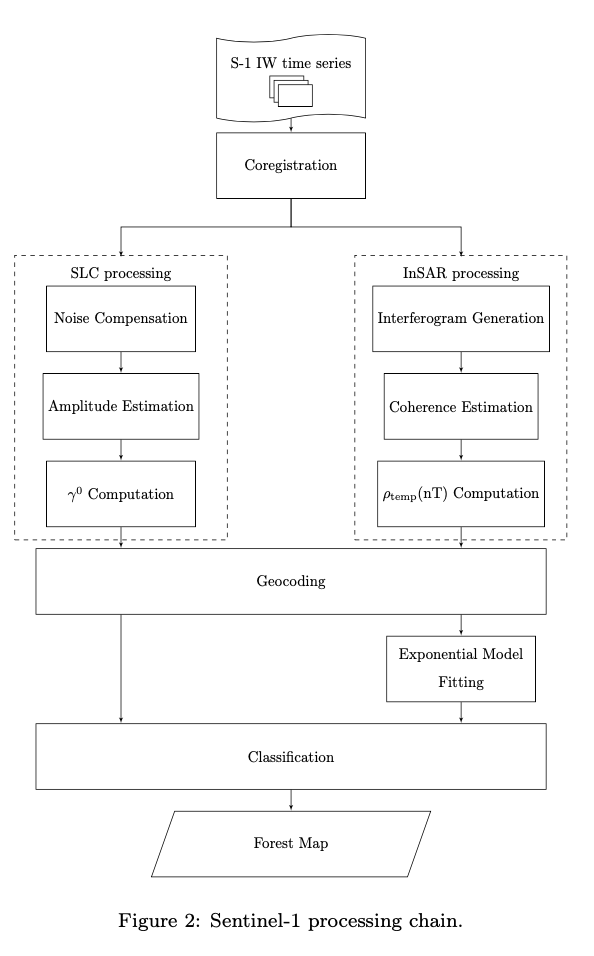
\includegraphics[width=0.7\linewidth]{Cap3/chain.png}
    \caption{Temporal Decorrelation for different decay factors \cite{Paolo}}
    \label{fig:processing_chain}
\end{figure}

After the coregistration there are two pipelines that must be implemented. The first pipeline deals with the SLC processing, and it is responsible to compensate the noise and estimate the backscatter. The second pipeline deals with the interferogram generation and estimation of coherence and temporal decorrelation.

After these two pipelines are properly dealt with, the geocoding step takes the image and makes a geometry transformation that lowers the resolution of the image - the resolution SENTINEL-1 is 3.7mX14m, but for computational purposes it is downgraded to 100mX100m. The geocoding is the step that transform the image coordinates from azimuth and range do latitude and longitude coordinates. 

After all that, it is finally possible to fit the decorrelation model for each pixel and extract the temporal decorrelation parameters for each pixel.

% (ADD FORMULAS FOR SLC PROCESSING?)
\section{Exponential model fitting}
\label{tresponto3}
In this part, after the geocoding was properly done, it is time to fit the exponential model curve with the data obtained. In the figure it is visually explained the combination of data that can be used for the exponential model fit. Since the data are acquired with a period of 6 days, there are some images that have a temporal baseline of 12 days between them, some with a temporal baseline of 18 days and so on. It was set a threshold of 30 days for the maximum temporal baseline for the interferogram generation. 

\begin{figure}[H]
    \centering
    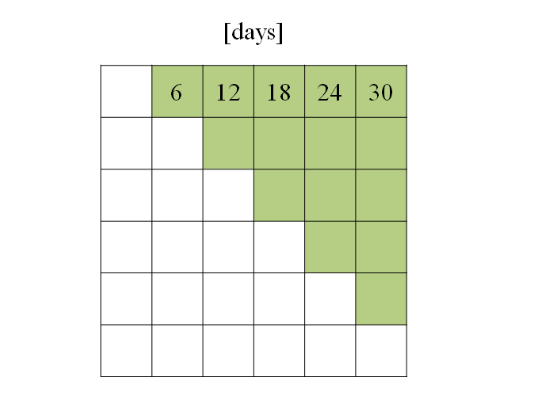
\includegraphics[width=0.7\linewidth]{Cap3/days.png}
    \caption{Available temporal baseline for exponential model fit \cite{Paolo}}
    \label{fig:days available}
\end{figure}

For each pixel $p$ on ground it is generated a tensor with the values of the temporal decorrelation for each of the available days - this tensor is here denoted $\rho_{temp} [n, i, j]$, where $n$ is the acquisition number ($n \in [1, N]$), $i \in [1, N-n]$ is the values for the temporal baseline $nT$ and $j$ is spatial dimension of a square neighbourhood ($\Omega(p))$ of size $L$ around that pixel.

After that tensor is created, the parameters are extracted by fitting the curve, that is done mathematically by minimizing the following functional:

\begin{equation}
    (\hat{\tau}, \hat{\rho_{LT}}) = arg min_{\tau, \rho_{LT}} \{
    \sum_{n=1}^N
    \sum_{i=1}^{N-n}
    \sum_{j \in \Omega(p)}
    (1-\rho_{LT}) \exp(-\frac{nT}{\tau})^2 + \rho_{LT} - \rho_{temp}[n,i,j]) 
    \}^2
\end{equation}

On practice this minimization was used with help of the Scipy library for Python. The Scipy library has a function which use non-linear least squares to fit a function to data available. 
\section{Feature Selection for Classification}
\label{tresponto4}

On this section it will be discussed the input features for the machine learning algorithm that was chosen to generate the classification map. The algorithm chosen was the Random Forest \cite{rf}, an algorithm based on decision trees that presented to be fast, flexible on the number of input parameters and provided a reasonable accuracy when compared to the references that exists for comparison. 

The Random Forest is an algorithm that even though it's recent, proved to be an effective tool for optical and SAR data \cite{rfsar}.

The input information that are possible to combine for the classification are: the backscatter coeficient, the decay correlation factor and the long term coherence. 

With that in mind it was applied three different inputs for the random forest:

\begin{itemize}
    \item backscatter only
    \item backscatter and long term coherence
    \item backscatter, long term coherence and decay factor
\end{itemize}

Another factor that is important to feed to the Random Forest is the incidence angle (the angle between the range and the normal on the ground) in which the SAR takes the acquisition. The incidence angle is important because it contains the topographical information, something that can alter the measurements of backscatter, therefore it is a parameter important for classification.

Different parameters were used for the classification map generation, in the end it was chosen the parameters that minimize the missclassification probabilty for the three classes (forest, nonforest and artificial surfaces).
\newpage
\section{Datasets used for validation}
\label{tresponto5}
The datasets were acquired via the Sentinel-1 interferometric wide swath (VV polarization channel) satellite. Each IW image has a resolution of 14m(azimuth direction) x 3.7m(range direction) and a period of acquisition of 6 days. 
The datasets used are the datasets over Germany and the Datasets over the Amazon rainforest. For validation it was used the Corine classification map \cite{corine} and the Prodes classification map \cite{prodes}.

The dataset over Germany comprises an area of over 700km x 500km. The Sentinel1 acquisitions information can be seen on the table below:
\\

\begin{table}[H]
  \resizebox{\textwidth}{!}{
  %
  \begin{tabular}{c c c c c c c c} 
     \hline
        & \textbf{Stack 1} & \textbf{Stack 2} &  \textbf{Stack 3} &  \textbf{Stack 4} &  \textbf{Stack 5} &  \textbf{Stack 6} &  \textbf{Stack 7}  \\ [0.5ex] 
     \hline
     \textbf{Orbit} & 139 & 139 & 139 & 168 & 168 & 168 & 168 \\
     \hline\hline
     \textbf{Image} & & & & \textbf{Acquisition Dates} & & & \\
     \hline
     1 & 2018.08.01 & 2018.08.01 & 2018.08.01 & 2018.07.28 & 2018.07.28 & 2018.07.28 & 2018.07.28\\
     2 & 2018.08.07 & 2018.08.07 & 2018.08.07 & 2018.08.03 & 2018.08.03 & 2018.08.03 & 2018.08.03\\
     3 & 2018.08.13* & 2018.08.13* & 2018.08.13* & 2018.08.09 & 2018.08.09 & 2018.08.09 & 2018.08.09\\
     4 & 2018.08.19 & 2018.08.19 & 2018.08.19 & 2018.08.15* & 2018.08.15* & 2018.08.15* & 2018.08.15*\\
     5 & 2018.08.25 & 2018.08.25 & 2018.08.25 & 2018.08.21 & 2018.08.21 & 2018.08.21 & 2018.08.21\\
     6 & 2018.08.31 & 2018.08.31 & 2018.08.31 & 2018.08.27 & 2018.08.27 & 2018.08.27 & 2018.08.27\\
     \hline
        & & & & \textbf{Corner Coordinates [deg]} & & & \\
    \hline
    lat min & 47.9676283 & 49.4508966 & 50.9358976 & 47.9499978 & 49.4358306 & 50.9199976 & 52.4016654\\
    lat max & 49.4748923 & 50.9608575 & 52.4458574 & 49.9545851 & 51.4413178 & 52.9263836 & 54.4098489\\
    lon min & 5.238333 & 5.5870266 & 5.9489214 & 9.3441662 & 9.6941661 & 10.0491661 & 10.4188564\\
    lon max & 8.9128063 & 9.3759577 & 9.8550366 & 13.1737098 & 13.6414315 & 14.1314738 & 14.6397917\\
     \hline
     
    \end{tabular}
%
}
  \caption{Description of Sentinel-1 data acquisitions over Germany. It is shown orbits information, geographical coordinates of acquisitions and date of acquisitions. The master image for coregistration is indicated on each stack with a *}\label{tab:label_test}
\end{table}

The Corine Classification Map comprises of 44 different classes and has a resolution of 100m x 100m over the Germany area. For our classification purposes only three classes are of interest: forest areas, non forest areas and artificial surfaces (one additional class for invalid data is also created for classification purposes only). The Corine classification map can be seen on the image \ref{fig:corine}.

\begin{figure}[H]
    \centering
    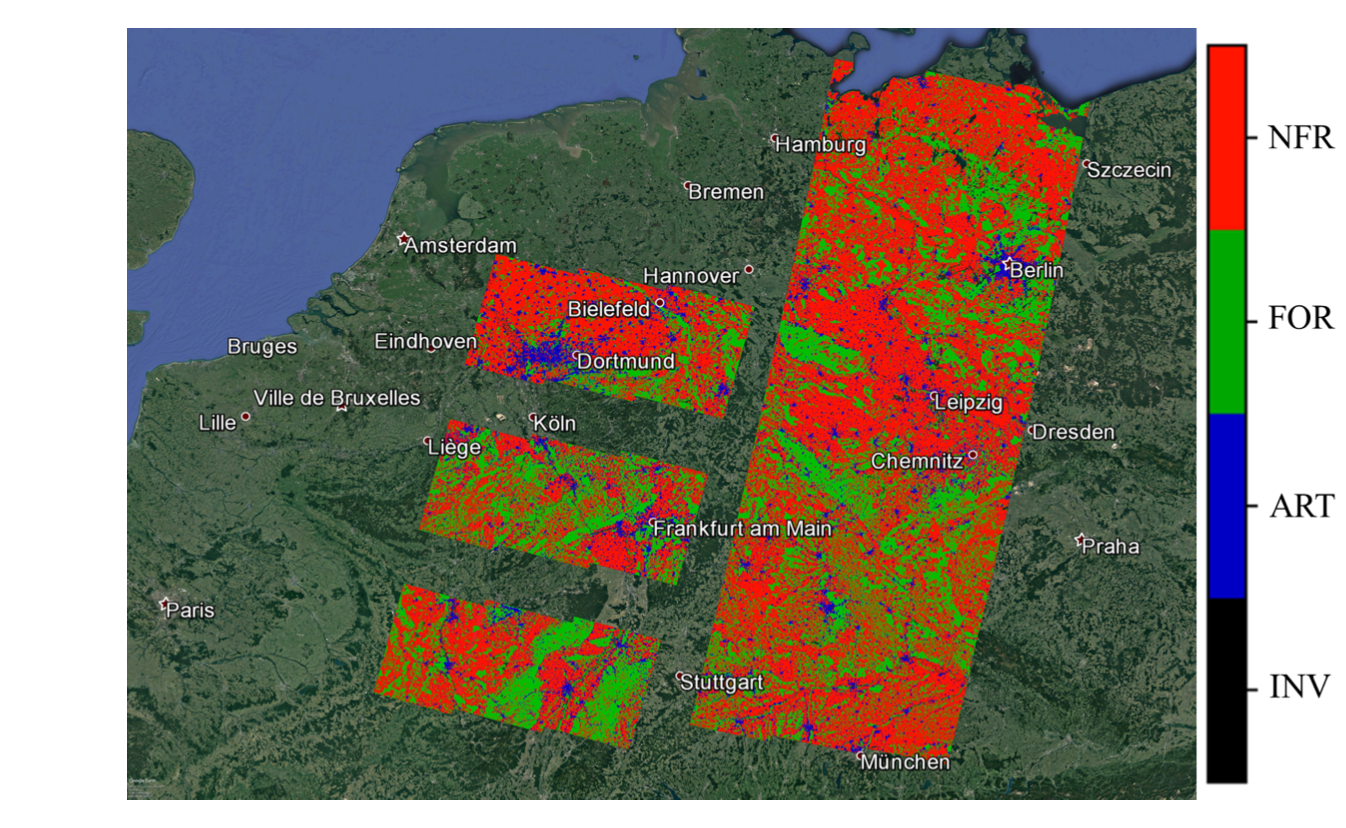
\includegraphics[width=0.7\linewidth]{Cap3/corine.png}
    \caption{Corine Reference Map from 2012 over Germany. The classes shown are non-forest areas (red), forest areas (green), artificial surfaces (blue) and invalid data(black)}
    \label{fig:corine}
\end{figure}

The area over the Amazon rainforest focuses primarely on the state of Rondonia, covering an area of over 238 $km^2$. This area was chosen because Rondonia is the main focus for deforestation on the Amazon Rainforest. The dataset consists of twelve short-time series acquisitions where each area was monitored 5 times. The time span in comparison to the master acquisition has a temporal baseline of 30 days. On the table below the acquisitions can be show in detail.

\begin{table}
  \resizebox{\textwidth}{!}{%
  
  \begin{tabular}{c c c c c c c} 
     \hline
     & & & \textbf{Coorner Coordinates} & &\\
     \hline
        \textbf{Stack} & \textbf{Orbit} & \textbf{Lat Min} & \textbf{Lat Max} & \textbf{Lon Min} & \textbf{Lon Max} &  \textbf{Acquisition Date}  \\ [0.5ex] 
     \hline
     1 & 010 & 9.405834S & 7.425399S & 59.5218.71W & 61.444320W &25/04/2019\\
     2 & 010 & 11.163674S & 9153141S & 60.125994W & 62.5152.W & 01/05/2019\\
     3 & 010 & 12.452109S & 10.432181S & 60.332320W & 62.262322W & 07/05/2019\\
     4 & 010 & 14.103267S & 12.124374S & 60.534814W & 62.465492W & 13/05/2019\\
     5 & 054 & 10.121596S & 8.44060S & 66.83473W & 67.594025W & 28/04/2019\\
     6 & 083 & 8.51951S & 6.505620S & 61.423210W &  63.36035W & 24/04/2019\\
     7 & 083 &  10.22836S & 8.325494S & 62.44436W & 63.373002W & 30/04/2019\\
     8 & 083 & 11.511677S & 10.22615S & 62.251509W &  64.19505W & 06/04/2019\\
     9 & 083 & 13.24387S & 11.324218 & S 62.443852W  & 64.403471W & 12/05/2019\\
     10 & 156 & 9.243467S &  8.41576S &  63.533037W &  65.56188W & 05/05/ 2019\\
     11 & 156 & 10.15776S &  8.483578S & 64.5705W &  66.82217W & 11/05/2019\\
     12 & 156 & 10.362114S &  9.462231S &  64.93968W &  66.19656W & 17/05/2019\\
     \hline
     
    \end{tabular}
%
}
  \caption{Description of Sentinel-1 data acquisitions over Amazon Rainforest. It is shown orbits information, geographical coordinates of acquisitions and date of acquisitions. }\label{tab:acquisitions_amazon}
\end{table}

For reference the PRODES (Programa de Cálculo do Desflorestamento da Amazônia) map was used. The reference map again  contains information about forest areas, nonforest areas and artificial surfaces. Figure \ref{fig:rondonia} shows the acquisitions over the Rondonia area.

\begin{figure}[H]
    \centering
    \includegraphics[width=0.7\linewidth]{Cap3/Rondonia.png}
    \caption{Prodes map over Amazon Rainforest. The classes shown are non-forest areas (red), forest areas (green), artificial surfaces (blue) and invalid data(black)}
    \label{fig:rondonia}
\end{figure}

\section{Accuracy Validation Methods}
It will be used two different accuracy measures to validate the results obtained: The overall accuracy and the average accuracy. Both these methods are valid for validating the model, but each one has its own advantage. The overall accuracy is primarily concerned trying to correctly classify the maximum number of pixels possible - without necessarily being concerned with creating a bias toward a certain class (normally these classifiers are biased toward the class that is most common in the data set). The average accuracy is concerned with trying to get a classifier that works well for all the classes possible on the data set and is calculated by averaging the classification results for each class. Below it is possible to see the mathematical formulas for calculating each accuracy.

\begin{equation}
    Overall\,Accuracy = \frac{Number\,of\,Pixels\,Classified\,Correctly}{Total\,Number\,of\,Pixels\, Available}
\end{equation}

\begin{equation}
    Forest\,Accuracy = \frac{Number\,of\,Forest\,Pixels\,Classified\,Correctly}{Total\,Number\,of\,Forest\,Pixels\, Available}
\end{equation}

\begin{equation}
    NonForest\,Accuracy = \frac{Number\,of\,NonForest\,Pixels\,Classified\,Correctly}{Total\,Number\,of\,NonForest\,Pixels\, Available}
\end{equation}

\begin{equation}
    ArtifialSurfaces\,Accuracy = \frac{Number\,of\,ArtifialSurfaces\,Pixels\,Classified\,Correctly}{Total\,Number\,of\,ArtifialSurfaces\,Pixels\, Available}
\end{equation}

\begin{equation}
    Average\,Accuracy = \frac{Forest\,Accuracy+NonForest\,Accuracy+ArtifialSurfaces\,Accuracy}{3}
\end{equation}

It is chosen also to use the abbreviations: OA (Overall Accuracy), FA (Forest Accuracy), NFA (NonForest Accuracy), AsA (Artificial Surfaces Accuracy) and AA (Average Accuracy).